

%  article.tex (Version 3.3, released 19 January 2008)
%  Article to demonstrate format for SPIE Proceedings
%  Special instructions are included in this file after the
%  symbol %>>>>
%  Numerous commands are commented out, but included to show how
%  to effect various options, e.g., to print page numbers, etc.
%  This LaTeX source file is composed for LaTeX2e.

%  The following commands have been added in the SPIE class 
%  file (spie.cls) and will not be understood in other classes:
%  \supit{}, \authorinfo{}, \skiplinehalf, \keywords{}
%  The bibliography style file is called spiebib.bst, 
%  which replaces the standard style unstr.bst.  

\documentclass[a4paper]{spie}  %>>> use for US letter paper
%%\documentclass[a4paper]{spie}  %>>> use this instead for A4 paper
%%\documentclass[nocompress]{spie}  %>>> to avoid compression of citations
%% \addtolength{\voffset}{9mm}   %>>> moves text field down
%% \renewcommand{\baselinestretch}{1.65}   %>>> 1.65 for double spacing, 1.25 for 1.5 spacing 
%  The following command loads a graphics package to include images 
%  in the document. It may be necessary to specify a DVI driver option,
%  e.g., [dvips], but that may be inappropriate for some LaTeX 
%  installations. 
\usepackage{amsmath}
\usepackage[]{graphicx}
\usepackage{hyperref}
\usepackage{listings}
\hypersetup{
    colorlinks,
    linkcolor={black!50!black},
    citecolor={blue!50!black},
    urlcolor={blue!80!black}
}
\usepackage{pdfpages}
\usepackage{parcolumns}

\usepackage[utf8]{inputenc} 
\usepackage[ngerman]{babel}
\usepackage[autostyle=true,german=quotes]{csquotes}

\usepackage{color}
\definecolor{lightgray}{rgb}{.9,.9,.9}
\definecolor{darkgray}{rgb}{.4,.4,.4}
\definecolor{purple}{rgb}{0.65, 0.12, 0.82}


\usepackage{array}
\newcolumntype{L}[1]{>{\raggedright\let\newline\\\arraybackslash\hspace{0pt}}m{#1}}
\newcolumntype{C}[1]{>{\centering\let\newline\\\arraybackslash\hspace{0pt}}m{#1}}
\newcolumntype{R}[1]{>{\raggedleft\let\newline\\\arraybackslash\hspace{0pt}}m{#1}}

\usepackage{xcolor,colortbl}
\usepackage{color}
\usepackage{float}
\definecolor{lightgray}{rgb}{.9,.9,.9}
\definecolor{darkgray}{rgb}{.4,.4,.4}
\definecolor{purple}{rgb}{0.65, 0.12, 0.82}

\lstdefinelanguage{JavaScript}{
  keywords={typeof, new, true, false, catch, function, return, null, catch, switch, var, if, in, while, do, else, case, break},
  keywordstyle=\color{blue}\bfseries,
  ndkeywords={class, export, boolean, throw, implements, import, this},
  ndkeywordstyle=\color{darkgray}\bfseries,
  identifierstyle=\color{black},
  sensitive=false,
  comment=[l]{//},
  morecomment=[s]{/*}{*/},
  commentstyle=\color{purple}\ttfamily,
  stringstyle=\color{red}\ttfamily,
  morestring=[b]',
  morestring=[b]"
}

\lstset{
   language=JavaScript,
   backgroundcolor=\color{lightgray},
   extendedchars=true,
   basicstyle=\footnotesize\ttfamily,
   showstringspaces=false,
   showspaces=false,
   numbers=left,
   numberstyle=\footnotesize,
   numbersep=9pt,
   tabsize=2,
   breaklines=true,
   showtabs=false,
   captionpos=b
}

\title{Smartphonecontroller Javascript-GameAPI}

%>>>> The author is responsible for formatting the 
%  author list and their institutions.  Use  \skiplinehalf 
%  to separate author list from addresses and between each address.
%  The correspondence between each author and his/her address
%  can be indicated with a superscript in italics, 
%  which is easily obtained with \supit{}.

\author{ Ron Schiwkowksi  (918691), Hannes Grothknopf (915449), Michael Schleiss (923739), Christian Heinrichs (919020), Dennis Hofmann (919285)
\skiplinehalf
University of Applied Sciences, Sokratesplatz 1, 24149 Kiel, Germany
}

%%%%%%%%%%%%%%%%%%%%%%%%%%%%%%%%%%%%%%%%%%%%%%%%%%%%%%%%%%%%% 
%>>>> uncomment following for page numbers
\pagestyle{plain}    
%>>>> uncomment following to start page numbering at 301 
%\setcounter{page}{301} 
 
  \begin{document} 
  \maketitle 
%%%%%%%%%%%%%%%%%%%%%%%%%%%%%%%%%%%%%%%%%%%%%%%%%%%%%%%%%%%%% 
\begin{abstract}
Lorem ipsum dolor sit amet, consetetur sadipscing elitr, sed diam nonumy eirmod tempor invidunt ut labore et dolore magna aliquyam erat, sed diam voluptua. At vero eos et accusam et justo duo dolores et ea rebum. Stet clita kasd gubergren, no sea takimata sanctus est Lorem ipsum dolor sit amet. Lorem ipsum dolor sit amet, consetetur sadipscing elitr, sed diam nonumy eirmod tempor invidunt ut labore et dolore magna aliquyam erat, sed diam voluptua. At vero eos et accusam et justo duo dolores et ea rebum. Stet clita kasd gubergren, no sea takimata sanctus est Lorem ipsum dolor sit amet.
\end{abstract}

%>>>> Include a list of keywords after the abstract 
\keywords{Smartphone, JavaScript, HTML5, Nodejs, API}

%%%%%%%%%%%%%%%%%%%%%%%%%%%%%%%%%%%%%%%%%%%%%%%%%%%%%%%%%%%%%
\section{Einleitung}
Lorem ipsum dolor sit amet, consetetur sadipscing elitr, sed diam nonumy eirmod tempor invidunt ut labore et dolore magna aliquyam.

\subsection{Problemstellung}
Lorem ipsum dolor sit amet, consetetur sadipscing elitr, sed diam nonumy eirmod tempor invidunt ut labore et dolore magna aliquyam erat, sed diam voluptua. At vero eos et accusam et justo duo dolores et ea rebum. Stet clita kasd gubergren, no sea takimata sanctus est Lorem ipsum dolor sit amet. Lorem ipsum dolor sit amet, consetetur sadipscing elitr, sed diam.
\begin{figure}[h!]
	\centering
		\fbox{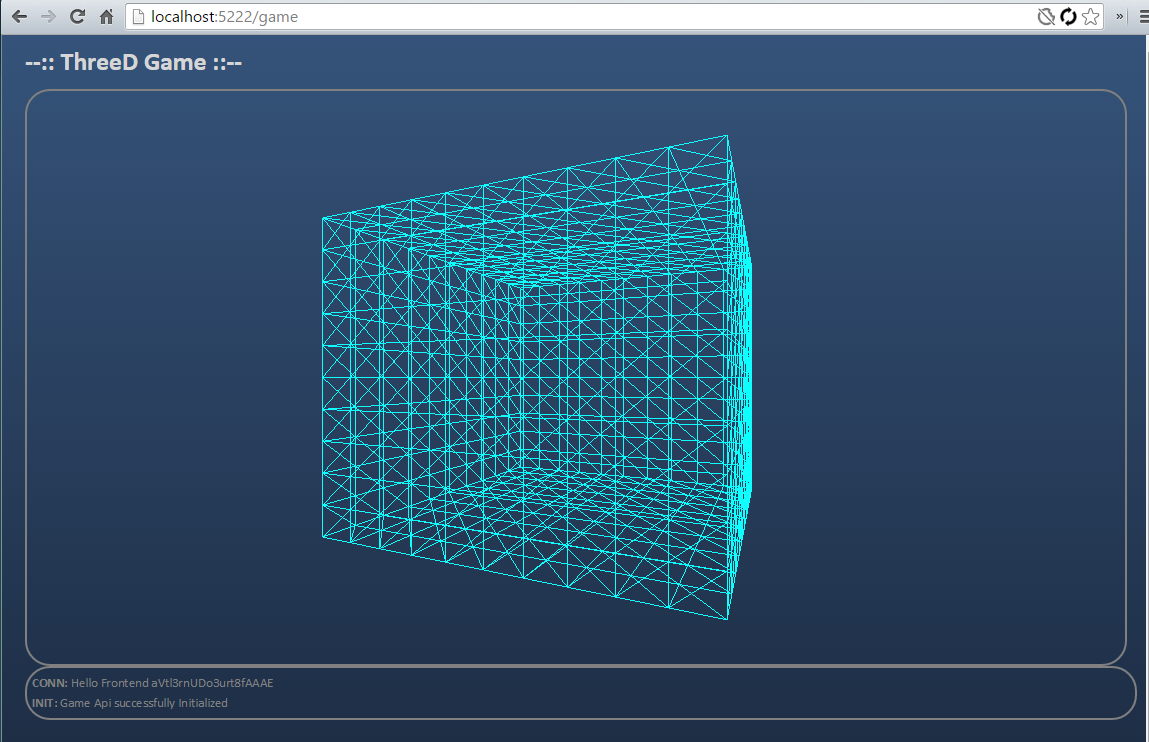
\includegraphics[width=12cm]{./images/FrontendInit.png}}
		\caption{Nicht ausgelastet Bar}
		\label{fig:FrontendInit}
\end{figure}

Lorem ipsum dolor sit amet, consetetur sadipscing elitr, sed diam nonumy eirmod tempor invidunt ut labore et dolore magna aliquyam erat, sed diam voluptua. At vero eos et accusam et justo duo dolores et ea rebum. Stet clita kasd gubergren, no sea takimata sanctus est Lorem ipsum dolor sit amet. Lorem ipsum dolor sit amet, consetetur sadipscing elitr, sed diam nonumy eirmod tempor invidunt ut labore et dolore magna aliquyam erat, sed diam voluptua. At vero eos et accusam et justo duo dolores et ea rebum. Stet clita kasd gubergren, no sea takimata sanctus est Lorem ipsum dolor sit amet.(siehe Abbildung \ref{fig:FrontendInit}).
\\
Lorem ipsum dolor sit amet, consetetur sadipscing elitr, sed diam nonumy eirmod tempor invidunt ut labore et dolore magna aliquyam erat, sed diam voluptua. At vero eos et accusam et justo duo dolores et ea rebum. Stet clita kasd gubergren, no sea takimata sanctus est Lorem ipsum dolor sit amet. Lorem ipsum dolor sit amet, consetetur sadipscing elitr, sed diam.

\section{Methodik}
\subsection{Projektmanagement}
Die Verteilung der Aufgaben ist in Tabelle \ref{table:distribution of tasks} aufgestellt.
Aufgaben sind im Gitlab erfasst und Personen zugewiesen. Ein wöchentliches persönliches Treffen aller Projektmitglieder führt zu einer guten Arbeitsmoral und hohen Effektivität.
\paragraph{GitLab}
Das Projekt wurde auf einem eigenen GitLab gehostet und den Projektmitgliedern zur Verfügung gestellt. Die Issues des Systems wurden genutzt um Aufgaben zu Verteilung und zu dokumentieren.\\
Strukuriert wurde das Arbeiten nach Feature Branches, um das Arbeiten am Projekt möglichst flexibel zu halten. Der Master-Branch diente als Release-Branch, in den regelmäßig die Änderungen per Merge Request eingetragen und getestet wurden.
\definecolor{blau}{HTML}{217AA2}
\begin{table}
	\label{table:Aufgabenverteilung}
	\centering
		\caption{Matrix distribution of tasks}
		\begin{tabular}{| L{2.6cm} | C{2cm} | C{2cm} | C{2cm} | C{2cm} | C{2cm} |}
		\hline
		\rowcolor{blau}
		\textcolor{white}{\textbf{Aufgabe}} & \textcolor{white}{\textbf{Schleiss}} & \textcolor{white}{\textbf{Grothknopf}} & \textcolor{white}{\textbf{Schiwkowksi}} & \textcolor{white}{\textbf{Hofmann}} & \textcolor{white}{\textbf{Heinrichs}}\\\hline
		Recherche 		& X & X	& X	& X	& X	\\\hline
		Konzept 		& X & X	& X	& X	& X	\\\hline
		Serverdesign	& 	& X & 	& X	& X \\\hline
		Networking		& 	& X	& 	& X	& X	\\\hline
		GameAPI 		& 	& X	&	&	& X	\\\hline
		DemoGame 		& X	&	&	&	& X	\\\hline
		ClientFrontend 	& X	&	& X	&	&	\\\hline
		ClientBackend 	& X	&	& X	&	&	\\\hline
		Database 	    & 	&	&	& X	& 	\\\hline
		LoginHandling   & 	& 	& 	& X	& 	\\\hline
		Poster          & 	& 	& 	& 	& 	\\\hline
		Documentation   & 	& 	& 	& 	& X \\\hline
		Projektmgmt. 	&	&	&	& 	& X	\\\hline
	\end{tabular} 
\end{table}

\subsection{Technologies}
\subsubsection{NodeJS}
Was ist NodeJS, Warum genutzt
\begin{figure}[h!]
	\centering
		\fbox{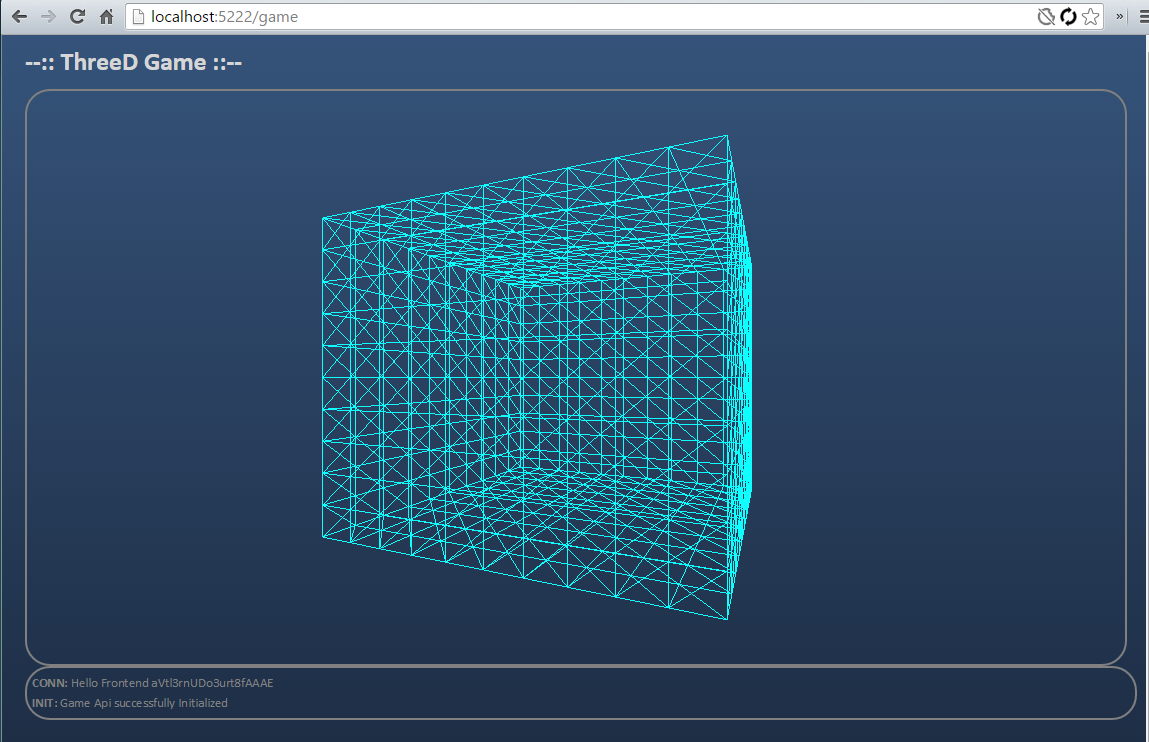
\includegraphics[width=12cm]{./images/FrontendInit.png}}
		\caption{Systemarchitektur WiFi Tracking}
		\label{fig:sysArch}
\end{figure}

Die Berechnung der Signalstärke wird nicht durch Kismet vorgenommen, sondern geschieht intern in der jeweiligen Netzwerkkarte. Es wird bei den Raspberry Pi ein LOGILINK WL0084B WiFi-USB-Stick verwendet. Die Dämpfung kann bei verschieden Netzwerkkarten stark abweichen. Deshalb ist es erforderlich, dass im Versuchsaufbau nur gleiche Netzwerkkarten verwendet werden.

\subsubsection{HTML 5}
Was kann HTML5, was nutzen wir für HTML 5 Features
\begin{figure}[h!]
	\centering
		\fbox{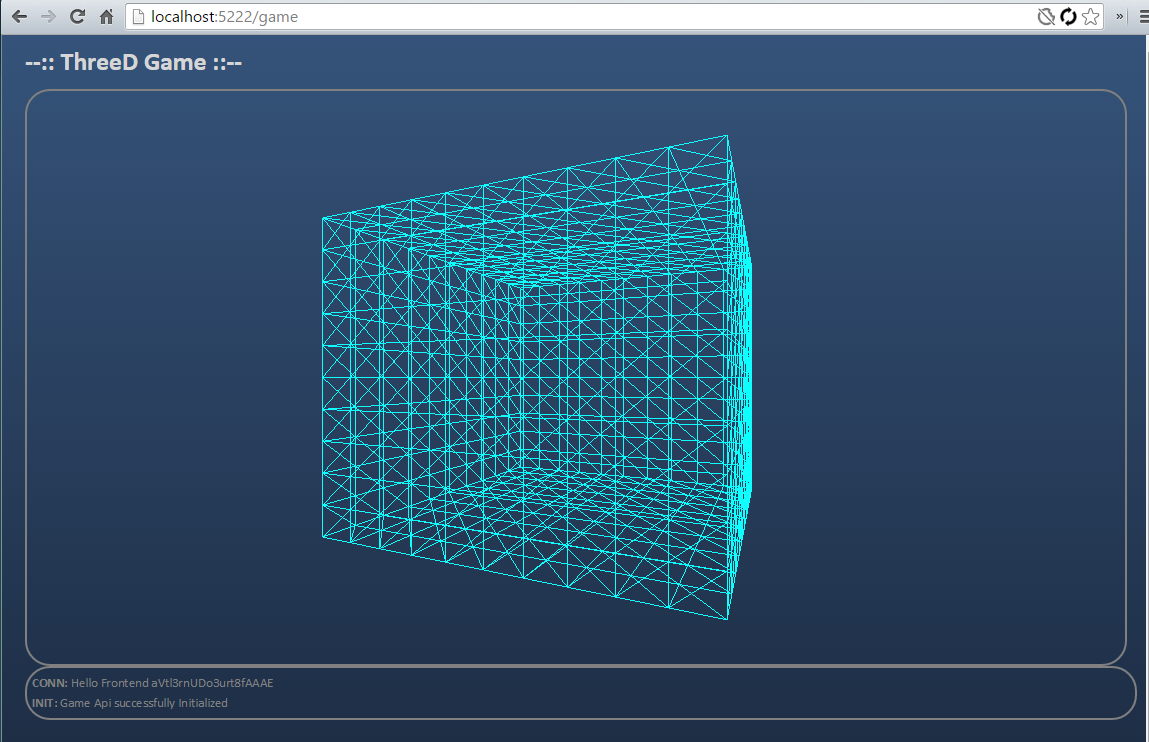
\includegraphics[width=10cm]{./images/FrontendInit.png}}
		\caption{Virtuelle Maschinen vs. Docker Container\cite{dockercontainer}}
		\label{fig:dockerVM}
\end{figure}

\subsubsection{Jacascript}
Was kann Javascript, ECMA 6
\begin{figure}[h!]
	\centering
		\fbox{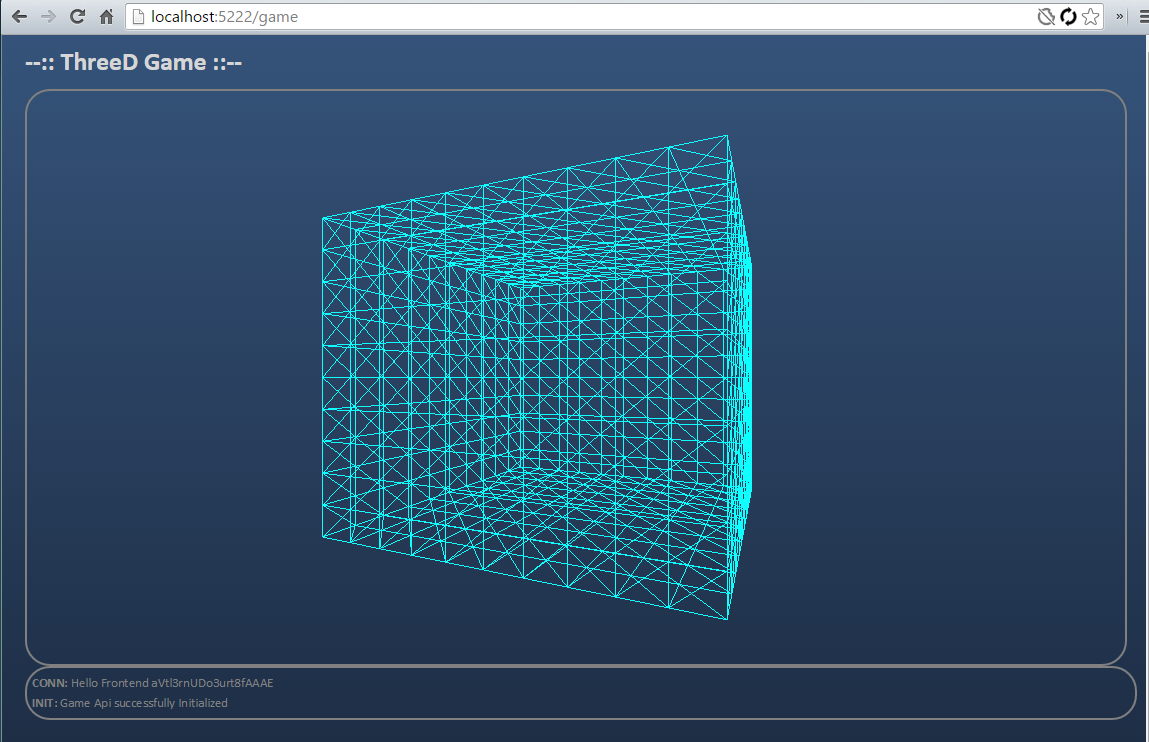
\includegraphics[width=10cm]{./images/FrontendInit.png}}
		\caption{Virtuelle Maschinen vs. Docker Container\cite{dockercontainer}}
		\label{fig:dockerVM}
\end{figure}
\subsubsection{MongoDB}
Was kann MongoDB, Warum MongoDB
\begin{figure}[h!]
	\centering
		\fbox{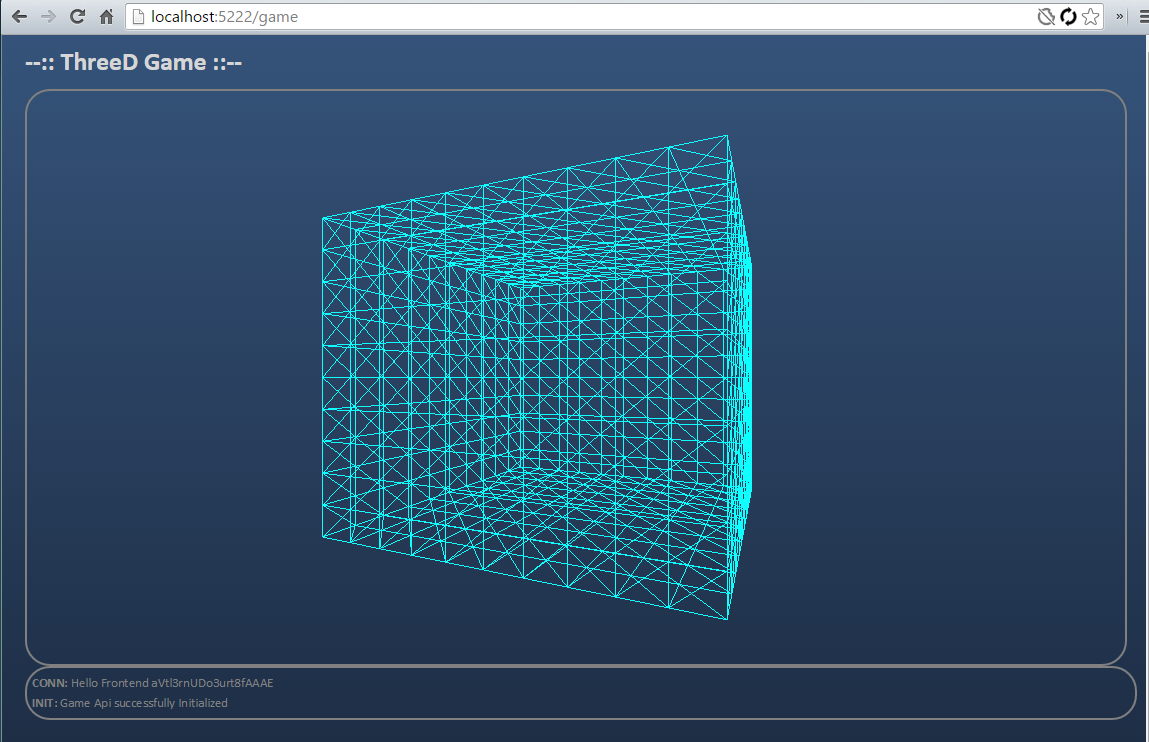
\includegraphics[width=10cm]{./images/FrontendInit.png}}
		\caption{Virtuelle Maschinen vs. Docker Container\cite{dockercontainer}}
		\label{fig:dockerVM}
\end{figure}
\subsubsection{Hardware}
Smartphone Controller, Platformunabhängig Node Server

%
% -----------------Implementation-------------------------
%

\section{Implementation}

\begin{figure}[h!]
	\centering
        \begin{lstlisting}[language=JavaScript,caption=Javascript Example]
           var a = 24;
           console.log(a);
        \end{lstlisting}
		\caption{Virtuelle Maschinen vs. Docker Container\cite{dockercontainer}}
		\label{fig:dockerVM}
\end{figure}

\subsection{User Management}
Das "UserManagement" kümmert sich um die Verwaltung der Nutzer. Dafür stellt es Funktionen für die Registrierung, Authentifizierung sowie für das setzen und holen von Benutzerdaten zur Verfügung. Die Funktionen im "UserManagement" bekommen eine callback Funktion übergeben, welche bei einer erfolgreichen Ausführung ausgeführt wird.

\subsection{Database}
Das "Database" Modul kümmert sich um die Persistente Speicherung aller anfallenden Daten. Dafür wird eine MongoDB verwendete und die für das hinzufügen, löschen, updaten und für Abfragen benötigten Funktionen zur Verfügung gestellt.


\subsection{API Beschreibung}
Hier wird die API Beschrieben!


\subsection{GameAPI}


\subsection{Demonstration}
\subsubsection{Preparations}


\subsubsection{Start applications}


\subsubsection{Running}


\section{Results}\label{result}
\subsection{Lasttestmessung}


\begin{figure}[H]
\begin{minipage}[t]{0.4\textwidth}
\vspace{0pt}
\paragraph{Struktur}\mbox{}\\
Der Versuchsaufbau wurde in direkter Nähe des WLAN Hotspots erstellt, um eine möglichst ideale Signalstärke zu erreichen. Der Versuchsaufbau besteht
\end{minipage}
\hfill
\begin{minipage}[t]{0.5\textwidth}
\vspace{0pt}
\centering
		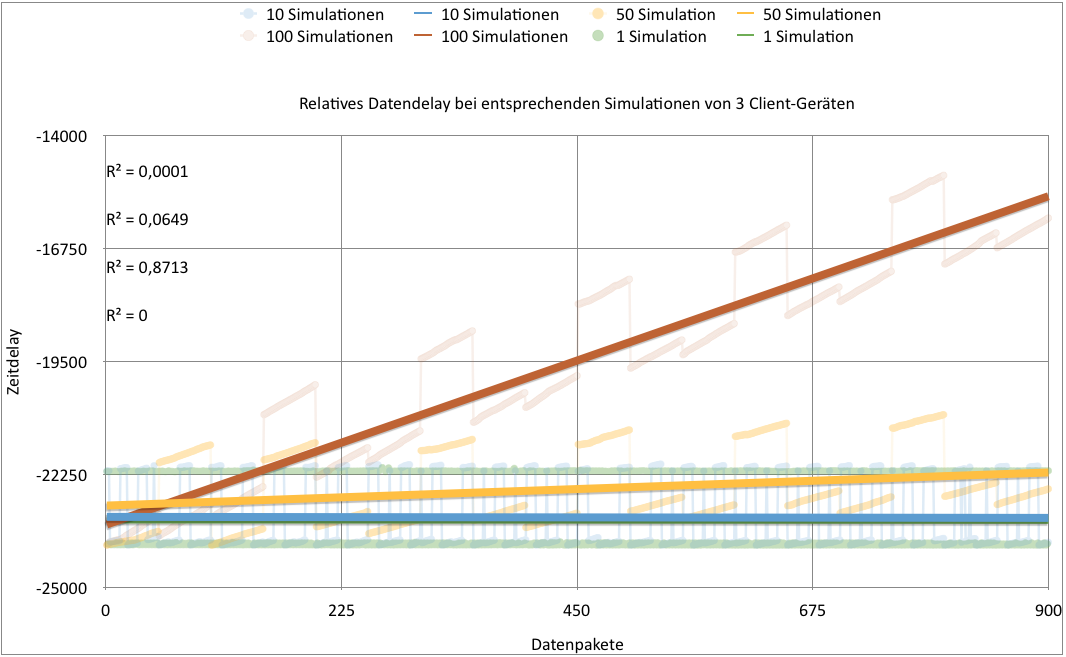
\includegraphics[height=5cm]{./images/LasttestDiagramm.png}
		\caption{Probemessung}
		\label{fig:probeMessung}
\end{minipage}
\end{figure}

\paragraph{Ablauf der Messung}\mbox{}\\
Anschließend wurde die in Abbildung \ref{fig:probeMessung} zur erkennende Strecke mit einem Smartphone abgelaufen. Beim Abgehen der Strecke wurde nach circa jedem Meter eine kurze Zeit verweilt, damit ein aussagekräftigeres Ergebnis erzielt werden konnte.

\paragraph{Results}\mbox{}\\
Auf Abbildung \ref{fig:test1} ist zu sehen von welcher Drohne sich das Gerät entfernt und welcher es sich nähert.\\

\begin{figure}[H]
\begin{minipage}[t]{0.4\textwidth}
\vspace{0pt}
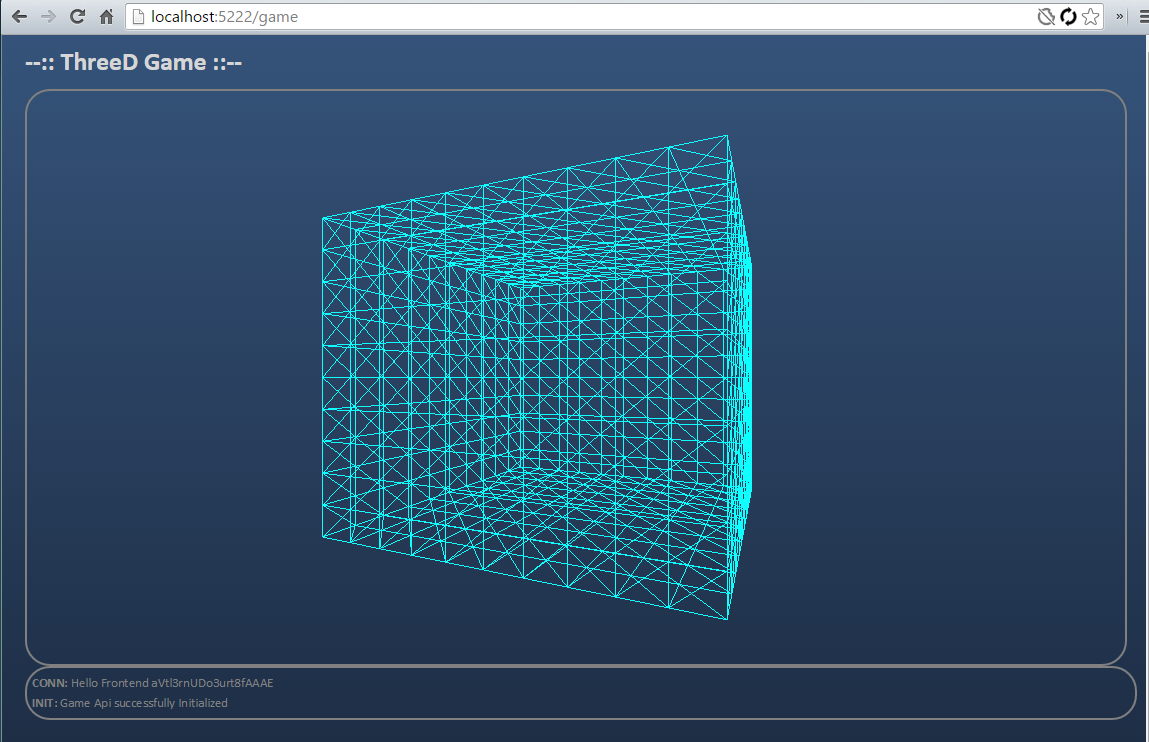
\includegraphics[height=5cm]{./images/FrontendInit.png}
\caption{Berechnungen zum Ergebnis}
\label{fig:tablleMessung}
\end{minipage}
\hfill
\begin{minipage}[t]{0.5\textwidth}
\vspace{0pt}
		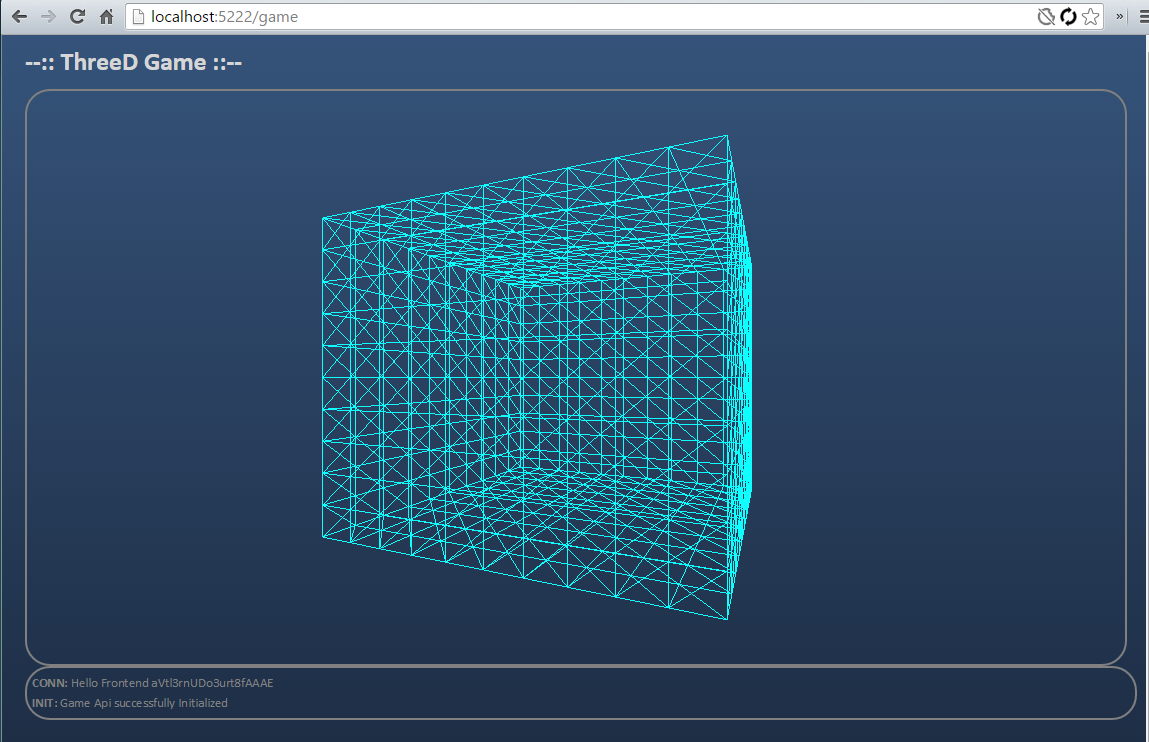
\includegraphics[width=\textwidth]{./images/FrontendInit.png}
		\caption{Ergebnis der Probemessung}
		\label{fig:test1}
\end{minipage}
\end{figure}

\subsection{Limitations}
\subsubsection{1. Test}

\paragraph{Ergebnis}\mbox{}\\
Selbst auf kurzer Distanz ist eine Differenz von ca. 10 dBm zwischen den Messpunkten zu sehen. Dies ermöglicht eine Ortsbestimmung auf kurzer Distanz, was beim nächsten Test ebenfalls zu sehen ist.

\begin{table}[H]
\centering
	\begin{tabular}{ | p{2.5cm} | l | l | l | }
		\hline 
		Entfernung	& 50 cm	& 100 cm	& 200 cm	\\ \hline
		Durchschnittliche Dämpfung & -62,22 dBm	& -75,45 dBm	& -82,52 dBm \\
		\hline
	\end{tabular}
	\caption{Ergebnisse des 1. Tests im störungsfreien Raum}
	\label{tab:probeTab}
\end{table}

\subsubsection{2. Test}\label{testNr2}

\begin{figure}[H]
\begin{minipage}[t]{0.4\textwidth}
\vspace{0pt}
\paragraph{Aufbau}\mbox{}\\
Um zu ermitteln, wie genau der Vergleich von Dämpfungswerten für die Positionsermittlung benutzt werden kann, wurden zwei Kismet-Drohnen in 12 Meter Abstand voneinander aufgestellt. Diese waren über einen Switch mit dem Kismet-Server verbunden. Alle 120 cm wurde ein Messpunkt festgelegt. Dies entsprach der Größe einer Bodenplatte im störungsfreien Raum und wurde deshalb als Distanz gewählt.
\end{minipage}
\hfill
\begin{minipage}[t]{0.5\textwidth}
\vspace{0pt}
		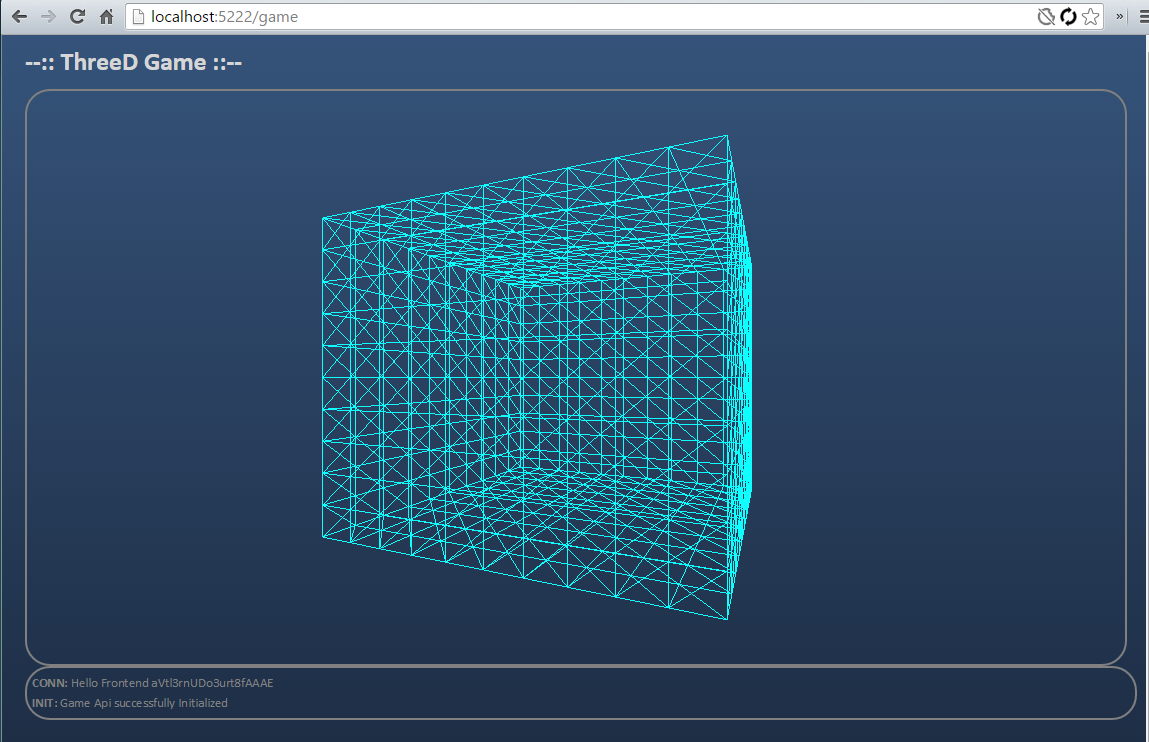
\includegraphics[width=\textwidth]{./images/FrontendInit.png}
		\caption{Aufbau 2. Test Störungsfreier Raum}
		\label{fig:test2}
\end{minipage}
\end{figure}

\paragraph{Ablauf der Messung}\mbox{}\\
Ein Smartphone wurde auf den entsprechenden Messpunkt gelegt. WiFi war auf dem Gerät eingeschaltet und die App zur Traffic-Generierung war aktiv. Es wurden pro Messpunkt circa 100 Messwerte aufgenommen, damit eine aussagekräftiges Ergebnis erzielt werden konnte und kurzzeitige Störungen abgefangen werden konnten.

\paragraph{Ergebnis}\mbox{}\\
Wie schon bei der ersten Probemessung ist eine deutliche Tendenz zu erkennen. Bei der Drohne, von der sich das Smartphone entfernte, nahm die Dämpfung zu. Bei der anderen Drohne nahm sie ab. Die aufgenommen Dämpfungswerte sind bei circa 480 cm gleich groß (siehe Diagramm \ref{fig:480} im Anhang). Dies ist 120 cm von der eigentlichen Mitte entfernt. Somit besteht eine Messungenauigkeit von 120 cm.

\subsection{Realistische Messung}
\paragraph{Aufbau}\mbox{}\\
Der Aufbau der Messung war der gleiche wie in der 2. Messung im störungsfreien Raum (siehe \ref{testNr2}). Dieses mal fand die Messung allerdings in einem einfachen Flur der FH-Kiel statt und war somit nicht vor Störungen geschützt.

\paragraph{Ablauf der Messung}\mbox{}\\
Ein Smartphone wurde an den einzelnen Messpunkten platziert. Das WiFi war auf dem Gerät aktiviert. Allerdings war das Gerät mit keinem WiFi-Netzwerk verbunden um die realen Umstände in einer Discothek nachempfinden zu können. Da von Anfang an festgestellt wurde, dass deutlich weniger Pakete abgefangen wurden, wurde die Dauer der Messung an jedem Messpunkt auf 2 Minuten festgesetzt.

\paragraph{Ergebnis}\mbox{}\\
Zu beobachten war, dass in den 2 Minuten 3-9 Pakete abgefangen wurden. Das macht eine Echtzeit-Bewegungsverfolgung so gut wie unmöglich. Ebenso war die Differenz der gemessenen Dämpfungswerte geringer, was eine Positionierung des Geräts erschwert. Das liegt daran, dass auf dem Flur Strahlen der WiFi-Antenne des Smartphones weniger stark gedämpft wurden. 




\section{Ausblick}

\paragraph{Glättung der Sensor Werte} Ein noch zu lösendes Problem ist die Glättung der von den Sensoren kommenden Werte. Je nach Gerät liefern die Sensoren unterschiedlich Stark schwankenden Daten. So feuert ein auf dem Tisch liegendes Gerät permanent Orientierungsdaten, obwohl es nicht bewegt wird. Diese Schwankungen müssen erkannt und unterbunden werden. Einbauen eines thresholds.


\paragraph{Disable touch zoom auf dem Client Gerät}
Beim wiederholten Klicken auf die Buttons der Client-Seite auf den Geräten wird unter Umständen in die Webseite gezoomt. Dies muss unterbunden werden um ein ungewolltes Verhalten zu unterbinden.


\paragraph{Begrenzung der gesendeten Sensor Daten}
Um den Server nicht ungleich durch die verschiedenen Geräte zu belasten, muss das Sendeverhalten reglementiert werden. Die optimalen Werte dafür müssen noch durch weitere Leistungstest ermittelt werden.



\section{Conclusion}
Alles super. Die erste Million ist nah!




%%%%%%%%%%%%%%%%%%%%%%%%%%%%%%%%%%%%%%%%%%%%%%%%%%%%%%%%%%%%%
%%%%% References %%%%%
\bibliographystyle{spiebib}   %>>>> makes bibtex use spiebib.bst
\bibliography{references}   %>>>> bibliography data in report.bib

\newpage
\appendix

\end{document} 
